\documentclass[UTF8]{article}
\author {Sherlock Liao}
\title {Programming Homework 4 }
\usepackage{amsmath}
\usepackage{amssymb}
\usepackage{graphicx}
\begin{document}
\maketitle
\section{Question}
For the periodic boundary question
$$
\begin{cases}
u_{t}=u_{xx}, \quad x \in [0,2\pi], t \geqslant 0 \\
u(x,0)=1+\sin(x)+\sin(10x), \quad x \in [0,2\pi]
\end{cases}
$$
\paragraph{}
(1)Using FTCS scheme to compute the value of u(x,t) at $t=0, 10^{-2}, 1$ and plot the picture. $\delta = \frac{\Delta t}{\Delta x^{2}} = \frac{1}{2}$, \quad N=100. Then let $\delta = 0.8$ and $\delta = 1$, compute the value of u(x,t) at $t=0, 10^{-2}, 1$ and plot the picture.Compare the difference and get the conclusion.
\paragraph{}
(2)Using BTCS scheme to compute the value of u(x,t) at $t=0, 10^{-2}, 1$ and plot the picture. $\Delta t = \Delta x$, $N = 100$. N is the number of space division.
\section{Algorithm}
\subsection{FTCS}
\paragraph{}
Here, using FTCS scheme, for every node, we can get the approximate formula
$$
v_{j}^{n+1} = v_{j}^{n} + \frac{\Delta x}{\Delta x^{2}}(v_{j+1}^{n} - 2v_{j}^{n} + v{j-1}^{n}) \quad j = 0,1,\dots,N
$$
and we have periodic boundary condition
$$
v_{j}^{n} = v_{j+N}^{n} \quad for 0  \leq n \leq \frac{T}{t_{n}}
$$
We can iterate, and get the numerical solution.
\subsection{BTCS}
\paragraph{}
We use BTCS scheme, and we can get the approximate formula
$$
v_{j}^{n+1} = v_{j}^{n} + \frac{\Delta x}{\Delta x^{2}}(v_{j+1}^{n+1} - 2v_{j}^{n+1} + v{j-1}^{n+1}) \quad j = 0,1,\dots,N
$$
Then we get the implicit scheme, and we can write in matrix form
$$
Av^{n+1} = v^{n}
$$
$$
A =
\begin{pmatrix}
    1+2 \delta & -\delta & 0 & \ldots & -\delta \\
    -\delta & 1+2 \delta & -\delta & 0 & \ldots \\
    \hdotsfor{5} \\
    -\delta & 0 & \ldots & -\delta & 1+2 \delta \\
\end{pmatrix}
$$
Then we can solve this linear equations by compute the inverse of matrix A, and then we can get the numerical solution by $v^{n+1} = A^{-1}v^{n}$
\section{Results and Analysis}
By coding, we can get the image below.

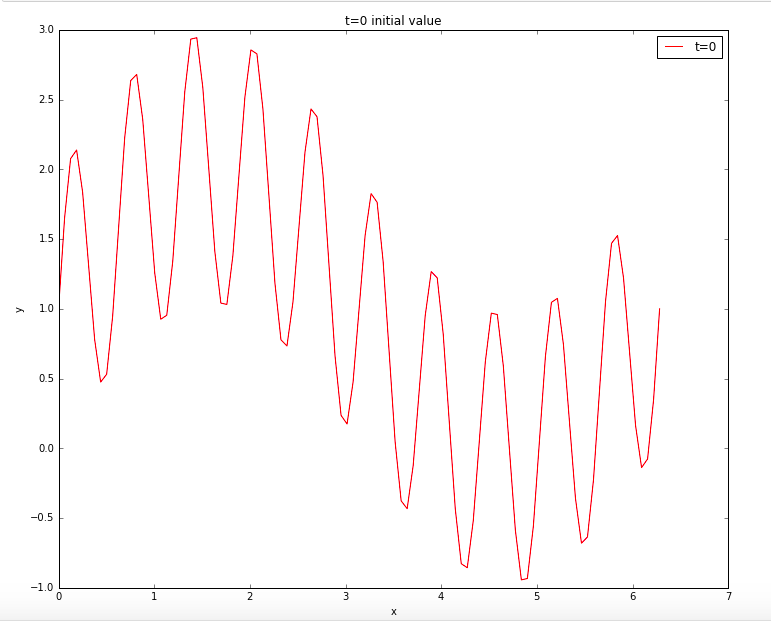
\includegraphics[width=10cm]{1.png}

\paragraph{}
First, we can get the value of the function at t=0. Whatever scheme, its initial value is the same, so we plot only one picture. We can see the result.

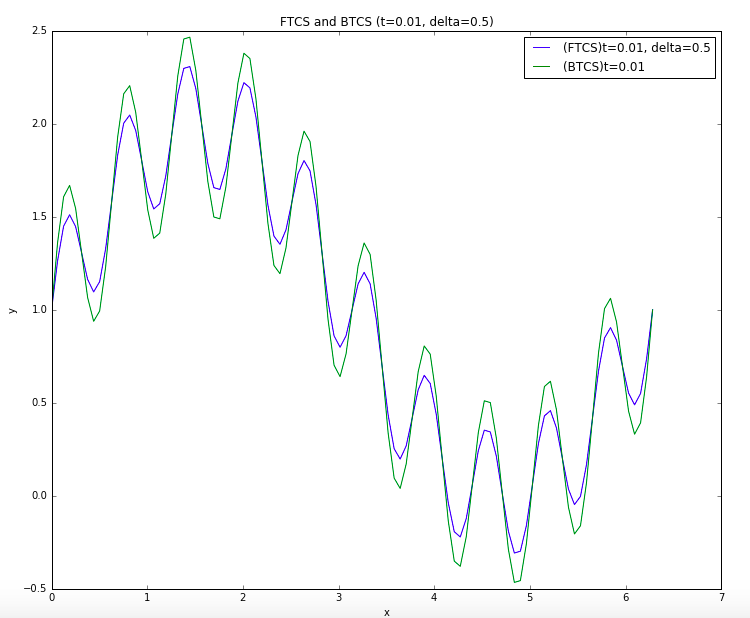
\includegraphics[width=10cm]{2.png}

\paragraph{}
For the second picture, we can compute the numerical solution at t=0.01 by using FTCS scheme and BTCS scheme. For the blue one, it's the FTCS's result when $\delta = 0.5$. For the green one, it's the BTCS's result. By the picture, we can see that there is a little different between the two results. At the bottom and top of the function values, there are some relatively big errors. For BTCS scheme, it has a larger swing than FTCS scheme.

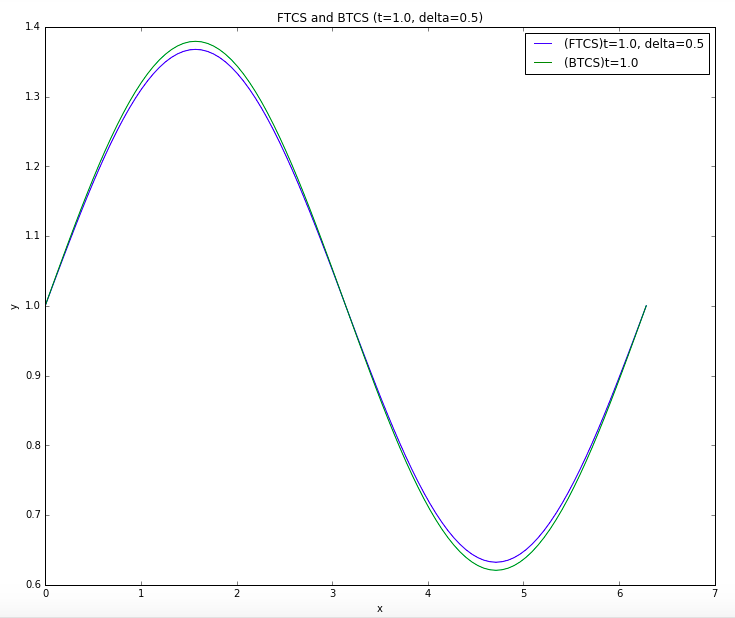
\includegraphics[width=10cm]{3.png}

\paragraph{}
For the third picture, it's the result at t=1.0 for FTCS and BTCS. We can see that both of them converge and have a good result. Again, BTCS scheme is more bias than FTCS. Maybe it's because BTCS is a implict scheme and it's unconditionally stable.

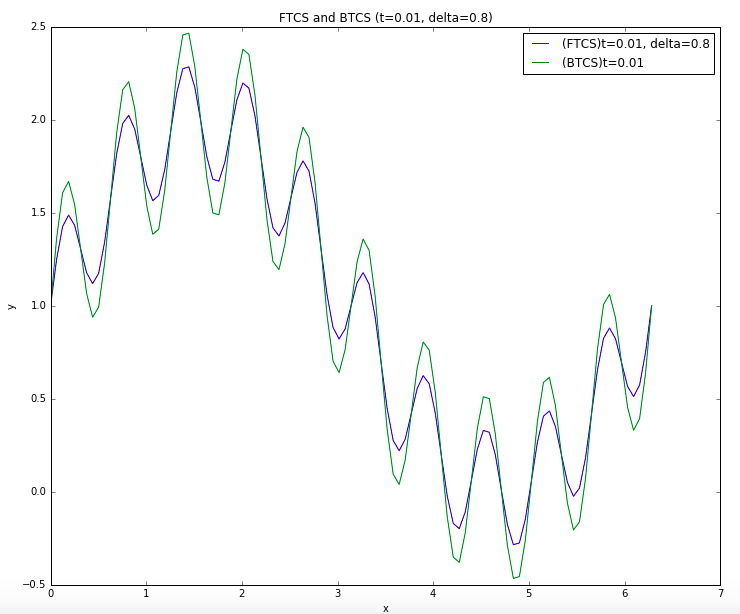
\includegraphics[width=10cm]{4.png}

\paragraph{}
For the forth picture, it's the result at t=0.01 when $\delta=0.8$, we can see that it's almost the same as the figure 1. So we can say that at t=0.01, they are the same.

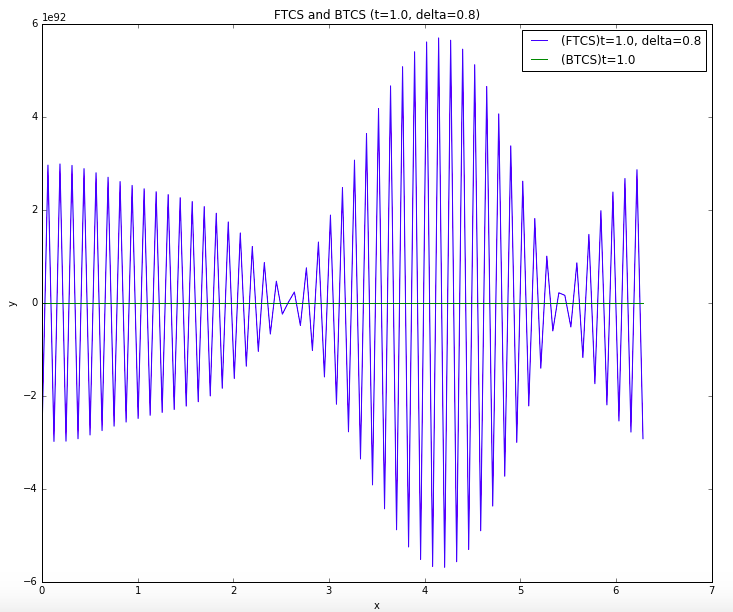
\includegraphics[width=10cm]{5.png}

\paragraph{}
From this picture, we can see that at t=1, the FTCS can't converge. We can get that FTCS's y is so large from the picture that it makes BTCS's y almost a line.

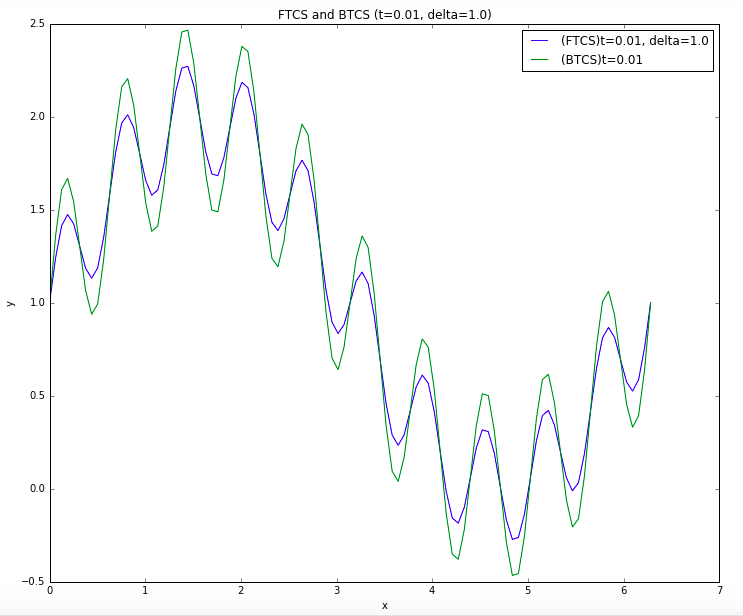
\includegraphics[width=10cm]{6.png}

\paragraph{}
From this picture, we get the result at t=0.01 when $\delta = 1.0$, it's also the same as $\delta = 0.5,0.8$ at t=0.01.

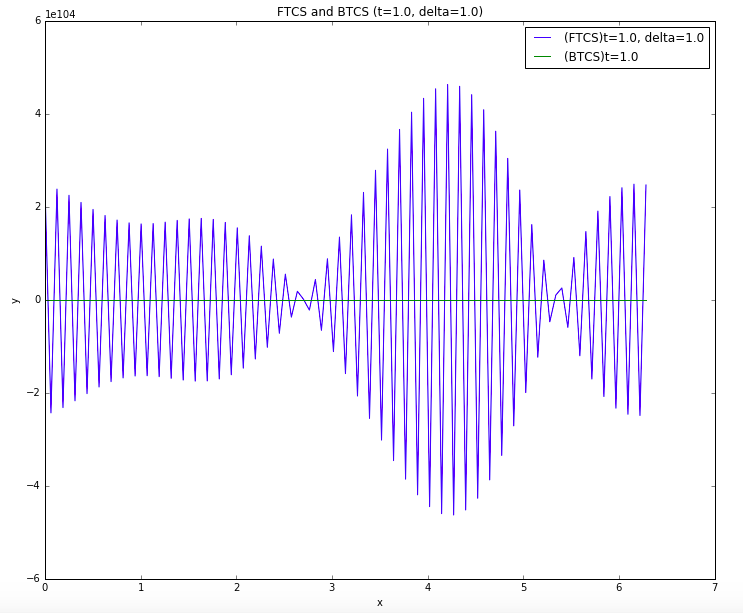
\includegraphics[width=10cm]{7.png}

\paragraph{}
This picture tells us the same result as Figure 5, and FTCS doesn't converge.

\paragraph{Summary}
Above all, we can see that because of BTCS is unconditionally stable, so it always has a good result. And for FTCS, if $\delta = 0.5$, we can get a good result, but if $\delta > 0.5$, such as 0.8 or 1.0 just like in the example, the result may not converge.

\end{document}
